% -----------------------------------------------
% chktex-file 44
\documentclass[../index.tex]{subfiles}

% -----------------------------------------------

\begin{document}

% -----------------------------------------------
\renewcommand{\sectiontitle}{Unicode}
\section{\sectiontitle}
% Moving from ASCII, we're going to examine Unicode, a standard created in the 1980s that now
% dominates the world.
%
% I hope you found ASCII pretty simple, because it's only going to get more complicated from a%
% technical perspective here on out.
%
% Why's that?
% Because text is complicated.

% ---------------------------
\renewcommand{\currenttitle}{The problems with ASCII}
\begin{frame}{\currenttitle}
% Let's review the problems with ASCII again.
% Knowing these shortcomings will help us understand how and why Unicode is designed the way
% it is.
%
% The original ASCII character set only supported the basic English alphabet, the ten Arabic
% numeral digits, some punctuations symbols, and some other unreadable symbols.
% As we've mentioned before, this isn't really going to cut it once you move outside of basic
% English.
%
% The extended ASCII character sets like Latin 1 tried to help this, but then we have many
% different widely adopted but largely incompatible character sets in different parts of the
% world.
% When you're transforming data across the globe into different systems using different
% character sets and encodings, this is going to be a problem.
%
% And as we'll see in a brief examination of other scripts, the terminology and design
% behind ASCII is too naïve to support many kinds of languages.
  Let's review: \\

  \begin{itemize}
    \item[--] Minimal language support
    \item[--] Variants that are widespread but incompatible
    \item[--] Too naïve for many types of languages
  \end{itemize}
\end{frame}

% ---------------------------
\renewcommand{\currenttitle}{Even more precise terminology}
\begin{frame}{\currenttitle}
\end{frame}

% ---------------------------
\renewcommand{\currenttitle}{How does Unicode define `character'?}
\begin{frame}{\currenttitle}
  ``The smallest component of written language that has semantic value; refers to the
    abstract meaning and/or shape, rather than a specific shape\ldots''
\end{frame}

% ---------------------------
\renewcommand{\currenttitle}{The Universal Character Set}
\begin{frame}{\currenttitle}
% Remember that the first component in handling text in the digital space is the character
% set.
% We have to define what characters we're handling, and to encode them, what numerical
% values we assign each one.
%
% The Unicode standard defines the Universal Coded Character Set (UCS) that contains most
% of the characters in most modern scripts.
% Every year, new characters are added to the set to increase coverage.
%
% The allowed codepoint values range from 0 to 10FFFF in hex.
% A portion of these codepoints are called surrogate codepoints (which we won't really talk
% about) so there are 1,112,064 possible codepoints.
% Many of the values are also unassigned to help make Unicode more future-proof and reduce
% conflicts with other encoding standards.
%
% Each character is also assigned a General Category that indicates that characteristics of
% that character.
% Some of the major categories include Letter, Number, Puntuation, Separator, etc.
\end{frame}

% ---------------------------
\renewcommand{\currenttitle}{The seventeen Unicode planes}
\begin{frame}{\currenttitle}
% These 1 million+ codepoints are split into seventeen 'planes', numbered 0 to 16.
% Each 'plane' is kind of like a semantic group.
%
% The first of these, plane 0, is the Basic Multilingual Plane, and contains characters for
% almost all modern languages.
% The codepoint values range from 0000 to FFFF, with some reserved values, resulting in a
% total of 65,472 allocated codepoints.
% Of those, 55,503 have been assigned a character.
%
% This includes Latin characters, other European scripts, Middle Eastern, African, South and
% Central Asian scripts, and others.
% Most of the codepoints are used to encode Chinese, Japanese, and Korean (CJK) characters.
%
% So most of the time, you're dealing with the Basic Multilingual Plane.
  \vspace*{1em}
  \begin{figure}
    \centering
    \includegraphics[width=0.8\textwidth]{\subdir/42-bmp.png}
    \caption{Basic Multilingual Plane}
  \end{figure}
\end{frame}

% ---------------------------
\renewcommand{\currenttitle}{The seventeen Unicode planes}
\begin{frame}{\currenttitle}
% The second plane is the Supplementary Multilingual Plane, or SMP.
% This contains historical characters and others that are general unused today.
%
% Examples include Linear B (the script used to write Mycenaean Greek), Egyption hieroglyphs,
% and cuneiform.
% This plane also includes musical and mathematical symbols, Emoji, and other pictographic
% sets.
  \vspace*{1em}
  \begin{figure}
    \centering
    \includegraphics[width=0.8\textwidth]{\subdir/42-smp.png}
    \caption{Supplementary Multilingual Plane}
  \end{figure}
\end{frame}

% ---------------------------
\renewcommand{\currenttitle}{Unicode encodings}
\begin{frame}{\currenttitle}
% Remember that Unicode defines the coded character set by assigning each character
% a codepoint.
% It doesn't specify which encoding you have to use to store these characters.
%
% The standard defines a few encodings, the most common of which are UTF-8 and UTF-16.
%
% The majority of websites are now encoded in UTF-8, and if you use a Unix-based system
% like Linux or macOS, the default encoding is UTF-8.
% For many modern programming languages, the encoding used internally for strings is UTF-8.
% In Rust, every string is handled internally as valid UTF-8.
%
% If you use Microsoft Windows, the default internal encoding is UTF-16.
% Java stores strings as UTF-16 internally.
%
% Of these, you should care the most about UTF-8. It's avoids complications found in
% UTF-16 and UTF-32 and is the most widely used encoding.
% The Web Hypertext Application Technology Working Group considers UTF-8 to be
% best practice and states that any browser application should not use UTF-16.
%
% So, we're going to focus primarily on UTF-8 and discuss UTF-16 briefly at the end.
  The Unicode standard defines a number of encoding formats:

  \begin{itemize}
    \item \textbf{UTF-8} \textendash{} 8-bit Unicode Transformation Format
    \item[] UTF-16LE \textendash{} 16-bit Unicode Transformation Format LE
    \item[] UTF-16BE \textendash{} UTF-16LE, but big-endian
    \item[] UTF-32LE \textendash{} 32-bit Unicode Transformation Format LE
    \item[] UTF-32BE \textendash{} UTF-32LE, but big-endian
  \end{itemize}
\end{frame}

% ---------------------------
\renewcommand{\currenttitle}{Examining UTF-8 encoding}
\begin{frame}{\currenttitle}
% Let's examine how characters are encoded and decoded to and from UTF-8.
%
% UTF-8 is a variable-width encoding, meaning each codepoint can take up a variable number
% of bytes.
%
% Characters are assigned codepoint values via the Universial Character Set, and we convert
% these values into binary to store in memory.
%
% In the case of UTF-8, each codepoint is stored as in 1, 2, 3, or 4 bytes.
% For example, the dollar sign, with a codepoint value of 36 (in decimal), takes up 1 byte.
% The Euro symbol, with a codepoint value of 8364 (in decimal), takes up 3 bytes.
% 4 bytes is enough to store every single character in the Universal Character Set.
%
% Unfortunately, as we'll see, we can't simply map the binary value directly to bits in
% memory like we did with ASCII.
% That's because this is a variable-width encoding.
% If we have a codepoint that takes up 2 bytes, followed by a codepoint that takes up 4 bytes,
% then 1 byte, we need to somehow know where each codepoint starts and ends.
%
% Thus, we put certain patterns of bits at the start of each byte to indicate how many
% bytes that codepoint takes up.
  UTF-8 is a \textbf{variable-width} encoding \\
  \vspace*{1em}
  Each codepoint is stored in \textbf{1 \textendash{} 4 bytes}

  \vspace*{1em}

  \begin{table}
    \begin{tabular}{c c c}
      Character & Codepoint   & Bytes required  \\ \hline
      \$        & \hex{0024}  & 1               \\
      ¢         & \hex{00A2}  & 2               \\
      €         & \hex{20AC}  & 3               \\
      𐍈         & \hex{10348} & 4
    \end{tabular}
    \caption{Number of bytes required to store certain characters}
  \end{table}
\end{frame}

% ---------------------------
\begin{frame}{\currenttitle}
% This table (basically stolen off Wikipedia) illustrates how this variable-width encoding
% works.
%
% The leftmost column indicates the number of bytes required.
% The second column indicates the range of codepoint values that are within that "category".
%
% As we can see from the first row, codepoints in the range 0x00 to 0x7F (0 to 127), inclusive,
% are stored in a single byte.
% Codepoints in the range 0x80 to 0x7FF (128 to 224), inclusive, are stored in a 2 bytes.
% And so on for 3 and 4 bytes.
%
% In the last 4 columns are the layout of bits in memory.
% The x's are placeholders for the actual bits of the codepoint values.
%
% First, let's look at the first row, the 1-byte case.
% A codepoint that requires 1 byte to encode takes up, of course, 1 byte.
% Notice that that byte always starts with the bit 0 and then has 7 placeholder x's.
% That's why only codepoints between 0 and 127, inclusive, can be stored in 1 byte.
%
% Thus, when we're decoding UTF-8, if we see that the first bit is 0, we know that this
% codepoint takes up only a single byte.
%
% Now the second row, the 2-byte case.
% The Byte 1 column indicates that the first byte of the 2-byte case always starts with the
% bits 110, followed by 5 bits that are the 5 most significant bits of the codepoint in binary.
%
% The Byte 2 column indicates that the second byte always starts with the bits 10, followed by
% the last 6 bits of the codepoint.
% So, if we see a byte that starts with 110, meaning any byte with a value between 192 and 223,
% inclusive, we know it's the first byte in a codepoint that takes up 2 bytes.
% Thus, we also know that the next byte must start with 10.
%
% To get the codepoint value, we simply extra the 5 bits in the first byte, and then append
% the 6 bits in the second byte.
% We could then convert that binary value into decimal or hex or whatever.
%
% It's a similar story for the 3-byte and 4-byte cases, except that the first byte starts
% with 1110 and 11110, respectively.
% Notice how every byte after the first in a group starts with 10.
%
% So, if we see a byte that starts with 1110, which is any byte with a value between 224 and
% 239, inclusive, we know it's the first byte in a 3-byte codepoint.
%
% If we see a byte that starts with 11110, which is any byte with a value between 240 and 247,
% inclusive, we know it's the first byte in a 4-byte codepoint.
% We also know that the next 3 bytes will start with 10, so we can extract the last 6 bits
% of each of those bytes and put them together.
%
% In the next slide, we'll look at a couple of examples to see how this plays out in practice.
  This table illustrates how bits are structured in the encoding: \\[1em]
  \begin{table}
    \scriptsize\ttfamily
    \begin{tabular}{rl llll}
      \#  & Range                         & Byte 1    & Byte 2    & Byte 3    & Byte 4    \\ \hline
      1   & U+0000\textendash{U+007F}     & 0xxxxxxx  &           &           &           \\
      2   & U+0080\textendash{U+07FF}     & 110xxxxx  & 10xxxxxx  &           &           \\
      3   & U+0800\textendash{U+FFFF}     & 1110xxxx  & 10xxxxxx  & 10xxxxxx  &           \\
      4   & U+10000\textendash{U+10FFFF}  & 11110xxx  & 10xxxxxx  & 10xxxxxx  & 10xxxxxx
    \end{tabular}
    \sffamily
    \caption{Layout of UTF-8 byte sequences}
  \end{table}
\end{frame}

% ---------------------------
\definecolor{darkgreen}{HTML}{5faf60}
\newcommand{\redc}[1]{\textcolor{red}{#1}}
\newcommand{\greenc}[1]{\textcolor{darkgreen}{#1}}
\newcommand{\bluec}[1]{\textcolor{blue}{#1}}
\newcommand{\magc}[1]{\textcolor{magenta}{#1}}
\begin{frame}{\currenttitle}
% Here's another table stolen off Wikipedia that uses some concrete examples to illustrate
% how these bits are laid out.
%
% In the first and second columns, we have the graphic representation of the character and
% the codepoint value (in hex) assigned to that character.
%
% In the third column, we have the binary representation of that codepoint value, and in
% the fourth column, how that binary is stored in UTF-8 encoding.
% The colors indicate which bits are stored in which bytes.
%
% Let's look at the dollar sign, whose codepoint value is 0x24, or 36.
% In binary, that's 100100.
% We can (and do) add a leading zero to that, which gives us 0100100. 7 bits.
% So, as we mentioned above, since 36 is less than 128, we can store the dollar sign in a
% single byte.
% As per the specification, our byte starts with a 0, and then we put the 7 bits of our
% codepoint.
%
% The cent symbol has a codepoint value of 0xA2, or 162.
% In binary, that's 10100010.
% 162 is greater than 128 and less than 224, so it takes 2 bytes to store.
%
% As per the specification, our first byte starts with 110, followed by the first 5 bits
% of our codepoint in binary.
% The second byte starts with 10, followed by the last 6 bits.
%
% In total, that's 11 bits.
% 10100010 is only 8 digits, so we add 3 extra leading zeros to make this value fit.
% Remember, in adding leading zeros, we're not changing the value of the codepoint.
%
% The first byte is 110, followed by the 5 first bits (which are in green): 00010.
% Thus, 11000010.
% The second byte is 10, followed by the last 6 bits (which are in red): 100010.
% Thus, 10100010.
% With that, we've encoded the cent symbol.
%
% To encode the euro and the hwair, which require 3 and 4 bytes, respectively, we do
% similar transformations.
% However, for the euro, the first byte will be 1110, followed by the first 4 bits,
% and for the hwair, the first byte will be 11110, followed by the first 3 bits.
  \begin{table}
    \tiny\ttfamily
    \begin{tabular}{c lr l}
      Char  & Hex         & Binary                    & UTF-8             \\ \hline
      \$    & \hex{0024}  & \redc{010 0100}           & 0\redc{0100100}   \\
      ¢     & \hex{00A2}  & \greenc{000 10}\redc{10}
                            \redc{0010}               & 110\greenc{00010}
                                                        10\redc{100010}   \\
      €     & \hex{20AC}  & \bluec{0010}
                            \greenc{0000 10}\redc{10}
                            \redc{1100}               & 1110\bluec{0010}
                                                        10\greenc{000010}
                                                        10\redc{101100}   \\
      𐍈     & \hex{10348} & \magc{0 00}\bluec{01 0000}
                            \greenc{0011 01}\redc{00}
                            \redc{1000}               & 11110\magc{000}
                                                        10\bluec{010000}
                                                        10\greenc{001101}
                                                        10\redc{001000}
    \end{tabular}
    \sffamily
    \caption{Representation of UTF-8 characters}
  \end{table}

% Here we have a bit table for the UTF-8 encoding of the euro symbol and then the dollar sign.
% If we read from left to right, we notice that our first bit starts with 1110. Thus, this
% first codepoint must take up 3-bytes.
% Notice how at positions 8 and 16, which are the start of the second and third bytes, it starts
% with the bits 10, as per the specification.
%
% So, we would extract the bits in positions 3 to 7, 10 to 15, and 18 to 23 to get the binary
% value of the first codepoint.
%
% We look at the remaining bytes.
% Position 24 is the start of the next byte, and we see that it starts with a 0.
% That means this next codepoint must take up only a single byte.
% To get the binary value, we take the bits in positions 25 to 31.
  \begin{figure}
    \footnotesize
    \begin{bytefield}{32}
      \bitheader{0,7,8,15,16,23,24,31} \\
      \bitboxes{1}{11100010 10000010 10101100 00100100}
    \end{bytefield}
    \caption{UTF-8 encoding of ``€\$''}
  \end{figure}
\end{frame}

% ---------------------------
\renewcommand{\currenttitle}{Writing a UTF-8 decoder}
\newcommand{\decoderheaderlisting}[2]{%
  \lstinputlisting[language=C++,captionpos=b,%
                   numbers=left,numbersep=8pt,
                   firstnumber=#1,
                   firstline=#1,lastline=#2]{%
    \codedir/utf8-decoder.hpp}%
}
\begin{frame}{\currenttitle}
% Hopefully that all makes sense.
%
% Let's write a UTF-8 decoder in C++. Don't worry if you don't know any C++, I'll walk through
% most of the code.
%
% We'll write a function convert a vector of UTF-8 encoded bytes into a vector of Unicode
% codepoints.
%
% Note that we won't be preforming any validation, so this is far from production-ready.
% We're simply assuming that the bytes are proper UTF-8.
%
% Here's part of our header file, where we'll define the function signatures and some constants.
%
% This is probably not a good practice, but we're going to alias unsigned char to a type called
% byte, and unsigned int to a type called codepoint.
% In C and C++, chars are 8-bit integers, and unsigned indicates that these values will always
% be positive.
% Thus, a byte, which we've defined as unsigned char, will simply be an 8-bit integer, representing
% an actual byte.
% Ints are 32-bit integers, so unsigned int denotes a positive 32-bit integer.
%
% We've given these names to make it clear that we're converting from a vectory of bytes to a
% vector of codepoints.
  Let's write a UTF-8 decoder in C++ \\

  We'll convert a vector of bytes into Unicode codepoints \\[2em]

  Our header file: \\[1em]

  \decoderheaderlisting{4}{7}
\end{frame}

% ---------------------------
% Here are the functions we'll be implementing.
%
% Let's look at the second one first.
% If you've ever written Java or any other C-family language, you'll probably realize that
% we've define the function 'decode' that takes in a vector of bytes, of unsigned 8-bit
% integers.
%
% A vector is similar to the ArrayList in Java and list in Python. It's simply a growable,
% ordered container of values.
%
% const lets us know that this function won't be modifying the vector that's passed in.
%
% And vector<codepoint> indicates that the function is returning a vector of codepoints,
% a vector of 32-bit unsigned integers.
%
% 'decode' will be the main function that we call to decode UTF-8 encoded bytes.
%
% Now let's look at the second one. This is a sort of auxilliary function that will help
% 'decode' perform its logic.
%
% We pass in an iterator to a vector of bytes and step through it until we've decoded a
% single codepoint. It'll modify the location of the iterator.
% 'end' is another iterator to the same vector that will tell us inside 'next_codepoint'
% if we've reached the end of the vector and there are no more bytes to process.
%
% 'next_codepoint' is going to return an optional, which is a sum type that contains a
% value or contains null. Think of it as something or nothing.
% We're returning either a codepoint, or we're returning nothing if we're in the middle
% of decoding an codepoint and we run out of bytes to process.
%
% Don't worry too much about some of the other details.
\begin{frame}{\currenttitle}
  Our function signatures: \\[1em]
  \decoderheaderlisting{1}{2}
  \decoderheaderlisting{14}{18}
\end{frame}

% ---------------------------
\begin{frame}{\currenttitle}
% Here are constants we'll use in 'next_codepoint'. We'll refer back to these later.
  Byte mask constants we'll use to help process each byte: \\[1em]
  \decoderheaderlisting{9}{12}
\end{frame}

% ---------------------------
\newcommand{\decodercodelisting}[2]{%
  \lstinputlisting[language=C++,captionpos=b,%
                   numbers=left,numbersep=8pt,
                   firstnumber=#1,
                   firstline=#1,lastline=#2]{%
    \codedir/utf8-decoder.cpp}%
}
\begin{frame}{\currenttitle}
% We'll start by implementing 'next_codepoint'.
% We'll be mutating the 'iter' iterator by consuming one or more bytes and converting
% it into an integer.
%
% Here we're first checking if we've already reached the end of the bytes.
% If so, we return an empty optional.
% Remember that the optional is like 'something' or 'nothing'.
% In this case, it's nothing.
  Check if the iterator has reached the end; if so, return nothing: \\[1em]
  \decodercodelisting{8}{13}
\end{frame}

% ---------------------------
\begin{frame}{\currenttitle}
% Let's start by handling the case where the next codepoint can be stored in a single
% byte.
% These are codepoints with values less than 128.
%
% We'll get the byte value the iterator is currently on and check if it's less than
% 128.
% Remember, this means that the most significant bit will be 0 and thus indicates
% that this codepoint takes up only a single bit.
% It also means that any valid 8-bit ASCII is also valid UTF-8.
%
% So, if it's greater than 128, the codepoint takes up more than a single byte, and
% have to write other code to handle that.
% But if it does happen to be less than 128, we consume the byte from the iterator by
% incrementing it.
% The next time we look at the iterator, it'll be pointing to the next byte value.
%
% Then, we'll simply cast the byte value into an unsigned 32-bit integer and return
% it.
  Handle the 1-byte case: \\[1em]
  \decodercodelisting{15}{21}
\end{frame}

% ---------------------------
\begin{frame}{\currenttitle}
% With the 1-byte case handled, let's handle the case where the codepoint is encoded in
% 2 bytes.
%
% In the 2-byte case, we remember that the first byte will start with the bits 110,
% and the second byte will start with the bits 10.
% That means the first bit must be less than 224, or 0xE0 in hex.
%
% We'll again first check if the iterator has reached the end of the byte stream and
% return nothing if it has.
%
% If not, we'll get the value of the next byte.
% This is the second byte in our 2-byte codepoint.

% We'll check if our first byte is less than 224.
% If so, we again increment the iterator to consume that byte.
%
% Since we're assuming that the byte stream we've been given is valid UTF-8, we're just
% assuming that the second byte starts with the bits 10.
% The next two lines do the decoding of the 2 bytes into a codepoint value.
%
% Remember, we can't simply convert these 2 bytes into integers and add or multiply them.
% When these bytes were encoded, the 5 most significant bits were taken and put in the
% first byte.
%
% We perform a bitwise AND operation on this first byte and the B2_MASK value defined in
% our header.
% This eliminates the leading 110 so we're left with 000 and then our first 5 bits,
% equal to just our first 5 bits.
% Then we cast this value into a unsigned 32-bit integer, so we have 27 leading 0's.
%
% Finally, by shifting the bits by 6 places, we drop the 6 most significant bits of this
% integer (which are all leading 0's) and add 6 least significant bits to the end.
% This leaves us with 6 0's following our 5 bits, and it's in those 6 spaces where we'll
% put the 6 bits decoded from the second byte.
% We store this in acc.
%
% In the next line, we perform another bitwise AND operation, this time on the second byte
% and the MB_MASK value defined in the header.
% We know the first 2 bits of the second byte are 10.
% We only care about the last 6 bits, so this operation eliminates those first two bits
% into 0's.
%
% Finally, the bitwise OR operation with acc puts these 6 bits into their place at the end
% of the codepoint.
% With that, we've successfully decoded the 2-byte case.
  Handle the 2-byte case: \\[1em]
  \decodercodelisting{24}{35}
\end{frame}

% ---------------------------
\begin{frame}{\currenttitle}
% Let's use an example to better understand the code we just went through.
%
% Suppose we have these two bytes (which we assume to be valid UTF-8): 11000010 10100010.
% We're not really sure what this decodes to yet, but let's find out.
%
% We read in the first byte (11000010), which has a value of 194.
% Since 194 is greater than 127 but less than 224, we know that this codepoint is
% a 2-byte case.
%
% Thus, we also read in our second byte (10100010).
%
% We know this is a 2-byte case, which means the first byte must start with the bits 110.
% As in the code, we perfrom a bitwise AND between our first byte and a mask of 00011111.
% If we manually go through each pair of bits and compute the AND operation, the first
% three bits (110) of our first byte become zero, and everthing else if left as is.
% So, we get 00000010.
%
% We cast this value to an unsigned 32-bit integer, so instead of 6 leading zeros, we have
% 30 leading zeroes.
%
% Next, we perform the bit shifting.
% We shift all the bits to the left by 6 positions, dropping any overflow and added zeros
% to the end.
% Our new value is equal to 10000000, with 24 leading zeros.
%
% Now, we handle the second byte (10100010).
% We know that the second byte, as per the UTF-8 specification, starts with the bits 10.
% By computing a bitwise AND operation between our second byte and a mask value of 00111111,
% we turn the leading 10 into 00, resulting in 00100010.
%
% We cast this value to a unsigned 32-bit integer to combine with our transformed first byte.
%
% The bitwise OR operation turns the last 6 0's in our transformed first byte into our
% transformed second byte, resulting in the final value of 10100010.
%
% 10100010 in decimal is 162, and 0xA2 in hex.
% This is the Unicode codepoint value for the cent symbol ¢.
  \begin{center}
    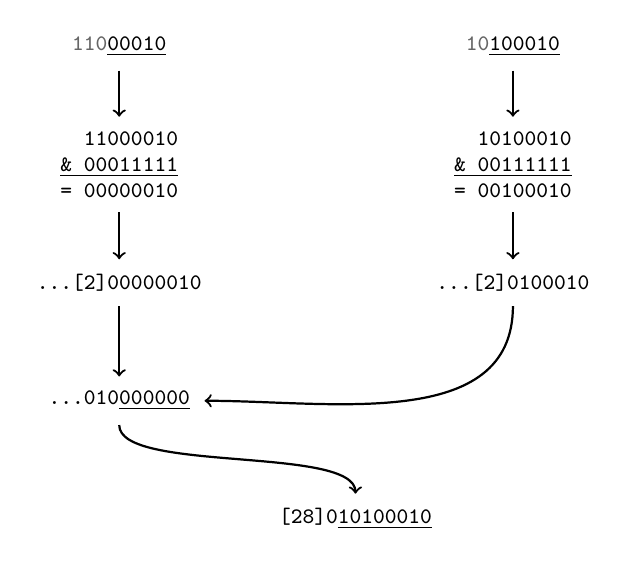
\begin{tikzpicture}[ampersand replacement=\&,%
      block/.style={%
        rectangle,
        align=center,
        outer sep=0.2em,
        font=\ttfamily\footnotesize,
      }]%
      \draw (0,0) node[block] (init0) {\textcolor{black!60}{110}\underline{00010}} ;
      \draw (0,-1.5) node[block, align=right] (mask0) {11000010 \\ \underline{\& 00011111} \\ = 00000010} ;
      \draw (0,-3) node[block] (cast0) {...\rpt[2]{0}0000010} ;
      \draw (0,-4.5) node[block, align=right] (shift0) {...010\underline{000000}} ;

      \draw [thick, ->] (init0.south) -- (mask0.north) ;
      \draw [thick, ->] (mask0.south) -- (cast0.north) ;
      \draw [thick, ->] (cast0.south) -- (shift0.north) ;

      \draw (5,0) node[block] (init1) {\textcolor{black!60}{10}\underline{100010}} ;
      \draw (5,-1.5) node[block,align=right] (mask1) {10100010 \\ \underline{\& 00111111} \\ = 00100010} ;
      \draw (5,-3) node[block] (cast1) {...\rpt[2]{0}100010} ;

      \draw [thick, ->] (init1.south) -- (mask1.north) ;
      \draw [thick, ->] (mask1.south) -- (cast1.north) ;

      \draw [thick, ->] (cast1.south) to[out=270,in=0] (shift0.east) ;

      \draw (3,-6) node[block] (final) {\rpt[28]{0}\underline{10100010}} ;
      \draw [thick, ->] (shift0.south) to[out=270,in=90,looseness=0.5] (final.north) ;
    \end{tikzpicture}
  \end{center}
\end{frame}

% ---------------------------
\begin{frame}{\currenttitle}
% Naturally, we next handle the 3-byte case.
%
% We do the same checks and get the value of the third byte.
% Then, since in the 3-byte case, the first byte must start with the bits 1110, we check
% if the first byte is less than 240, or 0xF0.
%
% If so, we consume the iterator and decode these 3 bytes.
%
% Similar to in the 2-byte case, we apply a bit mask using the bitwise AND operator to the
% first byte.
% In this case, our mask is the B3_MASK value we defined earlier rather than B2_MASK.
% This operation turns the four most significant bits, the 1110, into 0's, because we only
% care about the last 4 bits.
% Then, we shift these bits to the left again, except this time by 12 positions.
%
% We know that the second and third bytes will start with the bits 10, so we use the MB_MASK
% again to turn those leading 2 bits into 0's for each byte.
% The second byte's value is shifted left 6 positions and combined with the accumulated
% value.
% Finally, we combine the third byte's value with the accumulator and return the final value.
%
% Thus, we have 4 bits from the first encoded byte, then 6 bits from the second byte, and
% our final 6 bits from the third byte.

  Handle the 3-byte case: \\[1em]
  \decodercodelisting{38}{50}
\end{frame}

% ---------------------------
\begin{frame}{\currenttitle}
% Handling the 4-byte case looks very similar to the previous logic.
% Since we're assuming valid UTF-8, if the first bit doesn't start with 0, 110, or 1110, we
% assume that it must start with 11110.
%
% For the first byte, we apply a bit mask again, except this time it's the B4_MASK that
% changes the first 5 bits into 0's.
% Since we have 18 bits (provided by the next three bits) to put at the end of the codepoint
% value, we shift this value by 18 positions.
% For the second, third, and fourth bytes, we use the MB_MASK and shift each value by 12,
% and 6 places.
%
% And with this, we've completed 'next_endpoint'.
  Handle the 4-byte case: \\[1em]
  \decodercodelisting{52}{66}
\end{frame}

% ---------------------------
\begin{frame}{\currenttitle}
% Let's put it all together in 'decode'.
%
% Remember that the caller passes in a vector of bytes that they want decoded into codepoint
% values.
%
% We create two iterators that we'll pass into 'next_codepoint', one that points to the start
% of the bytes, and another that points to the end of bytes.
% In a loop, we call 'next_codepoint' repeatedly and append the result of each call to a
% vector that we return at the end of the function.
  Implementing \texttt{decode}: \\[1em]
  \decodercodelisting{68}{82}
\end{frame}

% ---------------------------
\begin{frame}[fragile]{\currenttitle}
% Here's a small function that creates a vector of bytes.
% Then, we pass it into decode to turn those bytes into codepoint values.
%
% We're passing the bytes in UTF-8 encoding for the cent symbol, the euro symbol, a Hangul
% syllable, and the hwair.
%
% This u8 syntax before the string literal in C++ tells the compiler to encode it in UTF-8,
% so that when we create our vector of bytes, it'll be bytes in UTF-8.
%
% If we call decode and print out the decimal values we get back, we can see that we get the
% correct codepoint values.
  \lstinputlisting[language=C++,numbers=left,numbersep=8pt,%
                   firstline=10]{\subdir/43-utf8.cpp}

  \vspace*{1em}

  The result:

  \input{\subdir/43-utf8.Rnw_tex}
\end{frame}

% ---------------------------
\renewcommand{\currenttitle}{UTF-16}
\begin{frame}{\currenttitle}
\end{frame}

% ---------------------------
\renewcommand{\currenttitle}{Unicode's shortcomings}
\begin{frame}{\currenttitle}
\end{frame}

% ---------------------------
\renewcommand{\currenttitle}{How to be Unicode-aware?}
\begin{frame}{\currenttitle}
\end{frame}

% ---------------------------
\renewcommand{\currenttitle}{Unicode in language X?}
\begin{frame}{\currenttitle}
\end{frame}

% -----------------------------------------------

\end{document}
